\chapter{Appendix: COMPAS arbiter survey design}\label{ch:appendix_softmono}

    \begin{figure}
        \centering
        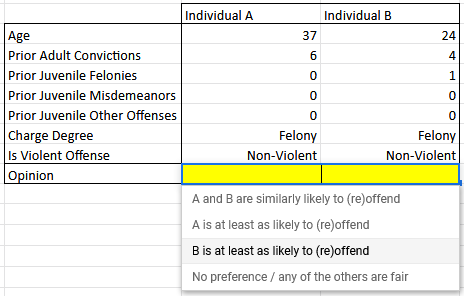
\includegraphics{fig_softmono/survey_form.png}
        \caption{Survey form used to collect arbiter ratings.}
        \label{fig:sm_survey_form}
    \end{figure}

    This supplement will discuss the collection of arbiter survey data as used in Section \ref{sec:softmono_experiments}. 
    
    Arbiters were \emph{not} collected at random, but volunteers known to the researchers.  They were given the following instructions, presented with 100 pairs of randomly drawn individuals from the COMPAS\cite{larson2016we} dataset, and asked to give one of four ratings in the form pictured in Figure \ref{fig:sm_survey_form}.  The following is the verbatim survey text given to volunteers.

    \begin{quote}
        DISCLAIMER: The survey below is ENTIRELY OPTIONAL and YOU CAN STOP AT ANYTIME.  Your answers are anonymous and will be combined in aggregate with others.  Your unaggregated answers will not be shared with anyone other than myself, and I will keep no record of who provided which answers.

        Your answers to this survey WILL NOT be used in any actual criminal proceedings (but please answer thoughtfully and honestly).
        
        BACKGROUND: Being granted bail allows an individual to leave jail between being arrested and facing prosecution; the individuals being considered have only been accused of an offense, not convicted, when their bail is set.

        Judges in the U.S. must assess whether an individual is likely to commit a crime if released on bail.  Some judges rely on computer models of past data to supplement their own intuitions and experience in making this determination.  These computer models have come under scrutiny for how "fair" their predictions are.

        The goal of this survey is to produce some example data on human judgments of what predictions would be "fair."  You'll be presented with a set of factors about two real defendants and asked to make a judgment about the what relative predictions would be "fair" for those individuals.
        
        The variables you are presented describe:
        - Age: what is the age of the person at time of setting bail (not age at time of alleged offense)
        - Prior Adult Convictions: how many prior crimes has the individual been convicted of as an adult
        - Prior Juvenile Felonies: How many felonies were they convicted of as juveniles.
        - Prior Juvenile Misdemeanors: How many misdemeanors were they convicted of as juveniles.
        - Prior Juvenile Other: How many other offenses, not counted as felonies or misdemeanors, were they convicted of as juveniles.
        - Charge Degree: Either Felony or Misdemeanor.  Felonies are considered more serious crimes and can carry longer prison sentences and higher fines.
        - Is Violent Offense: We have categorized the charged offenses as being Violent or Non-Violent based on the FBI's uniform crime reporting (UCR) standard: "violent crime is composed of four offenses: murder and nonnegligent manslaughter, forcible rape, robbery, and aggravated assault. Violent crimes are defined in the UCR Program as those offenses which involve force or threat of force.
        
        For each individual, please select 1 of 4 opinions from the highlighted drop down list:
        - "A and B are similarly likely to (re)offend"- You believe that Individuals A and B should have similar predicted likelihood to commit an offense while on bail.
        - "A is at least as likely to (re)offend" - You believe that Individual A can't fairly be predicted to have a lower chance of committing an offense while on bail.
        - "B is at least as likely to (re)offend" - You believe that Individual B can't fairly be predicted to have a lower chance of committing an offense while on bail.
        - "No preference / any of the others are fair" - It wouldn't be unfair if either individual had a higher, lower, or similar prediction to the other.
    \end{quote}
